We chose 3 different benchmarks for CPU in MiBench benchmark suite. We run them in 3 CPU frequencies and obtain power, performance, and temperature results. These results provide baseline profiles for our future work. 

\paragraph{Benchmarks}


We choose memory-intensive (jpeg), compute-intensive (bitcount), and a balanced (stringsearch) benchmarks from MiBench. In the previous report, we proposed to use SPLASH2 \cite{woo1995splash} benchmark suite. However, we changed it to MiBench and more daily usage benchmarks such as stringsearch which is an office benchmark. Our motivation to choose these benchmarks is doing meaningful work while running DNN on GPU. Hence, one may use CPU to run office programs while running a DNN inference on GPU. 

\begin{figure}
  \caption{Characteristics of chosen CPU benchmarks.}
  \centering
    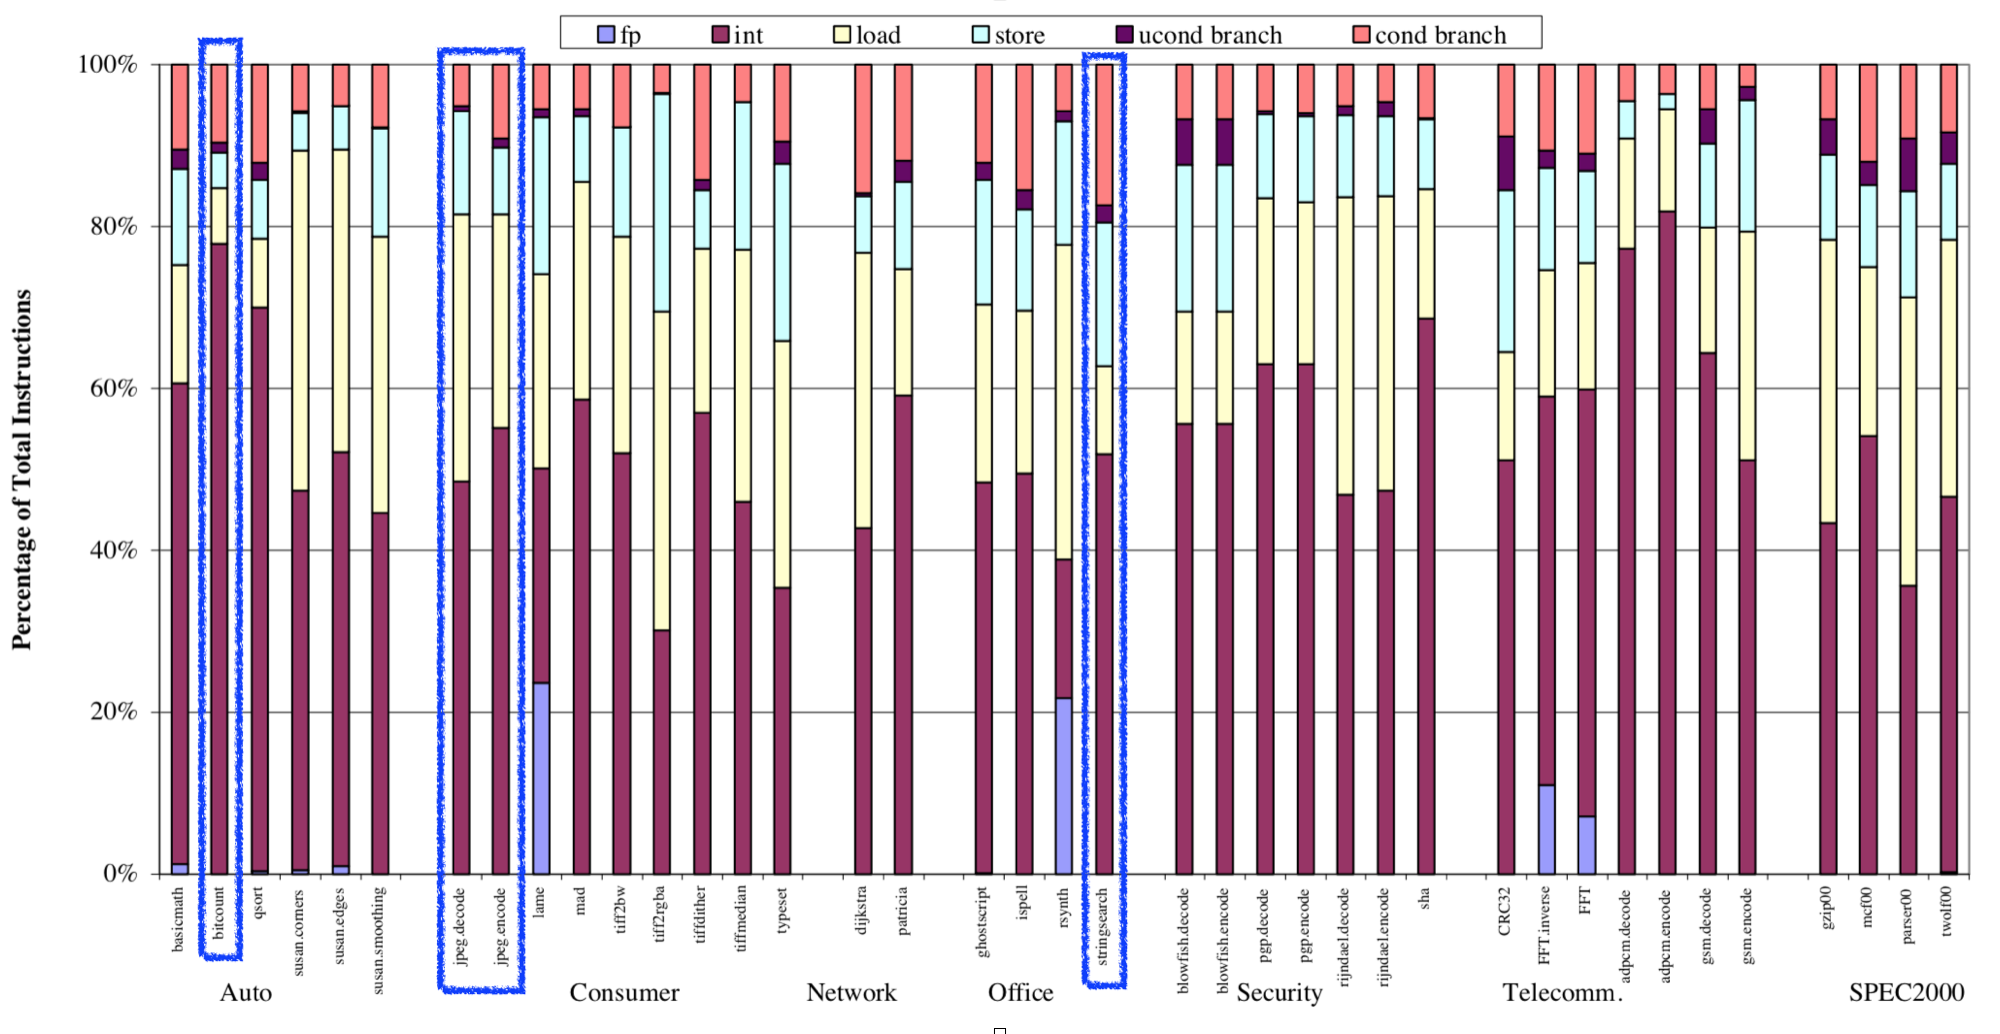
\includegraphics[width=0.5\textwidth]{cpubench}
\end{figure}

We run these benchmarks at 3 different frequency values which are the lowest (102 Mhz), the highest (1.73 Ghz), and the middle (921.6 Mhz) available frequency values for CPU. 

\paragraph{Profiling}


We run aforementioned 3 benchmarks with 3 different frequency values for CPU while not running anything on GPU to obtain a baseline for CPU. We calculate power, performance, and temperature results for CPU. 

\begin{figure}[h]
    \centering
    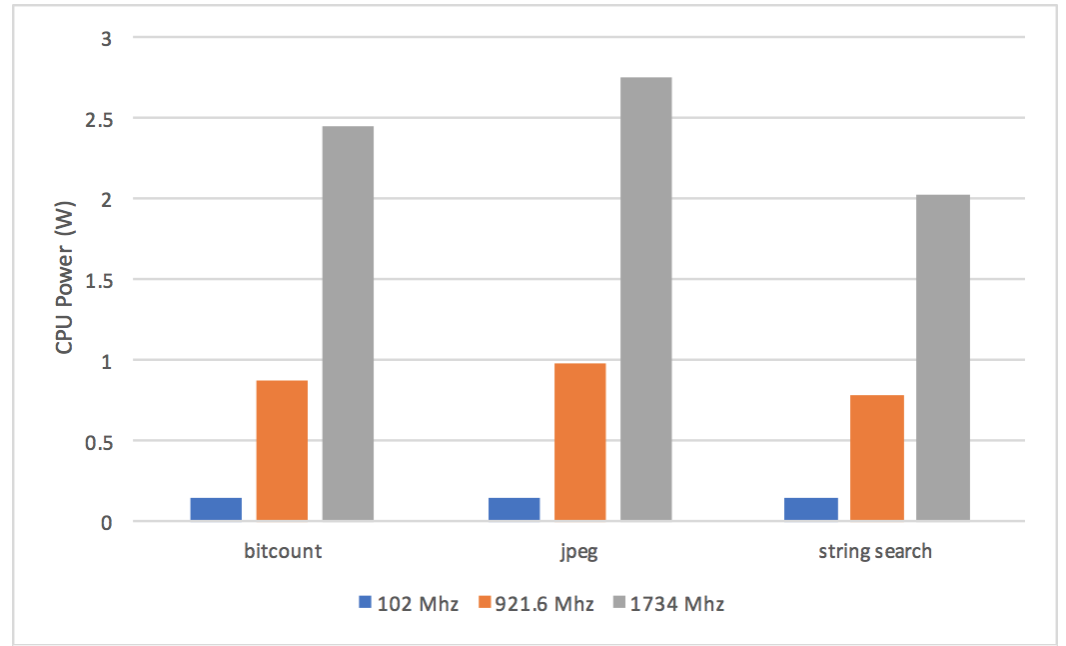
\includegraphics[width=0.5\textwidth]{cpupower.png}
    \caption{The power profile when running CPU benchmarks under different CPU voltage/frequency pairs.}\label{fig:cpupower}
\end{figure}

We calculate power using sensors in TX1 board as it is shown in Figure 5. One of the observations is that power increases as we increase CPU frequency. Another important observation is that power consumption is the highest for jpeg benchmark which is an image compression and decompression workload. Furthermore, the lowest power consumption comes from stringsearch benchmark which is an office workload. 
Moreover, we calculate temperature (Celcius) by using thermal sensors in TX1 board. Figure 6. shows temperature profile of CPU and GPU while running CPU benchmarks with various frequency values. Temperature results also follow the same trend with power results. In addition, GPU temperature also follows the same trend with CPU temperature since GPU does not run anything and CPU temperature affects GPU temperature. 
We also obtain performance results by using instruction per cycle (IPC) metric and CPU utilization for each frequency and benchmark pairs. Figure 7. shows IPC and CPU utilization results for each benchmark and frequency values. Results show that IPC value does not change when we change frequency values. Furthermore, CPU utilization is also at almost 100\% for bitcount and jpeg benchmarks. However, CPU is only 83\% at 102 Mhz and it becomes 44\% at 1.73 Ghz. It shows us that stringsearch benchmark does not need as much CPU resources as other benchmarks. 
Another significant conclusion is that IPC value of bitcount is higher than jpeg benchmark. However, power consumption of jpeg is higher than bitcount benchmark. It reveals that jpeg uses more power consuming instructions.


\begin{figure}[h]
    \centering
    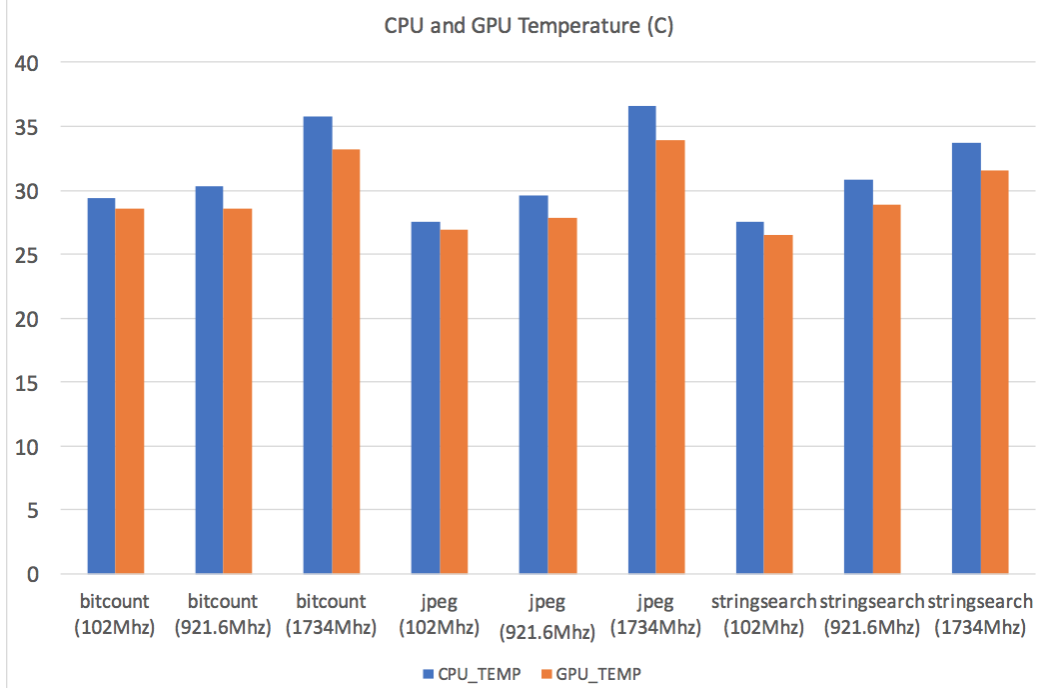
\includegraphics[width=0.5\textwidth]{cputemp.png}
    \caption{The temperature profile of CPU and GPU while running CPU benchmarks under different CPU voltage/frequency pairs.}\label{fig:cputemp}
\end{figure}


\begin{figure}[h]
    \centering
    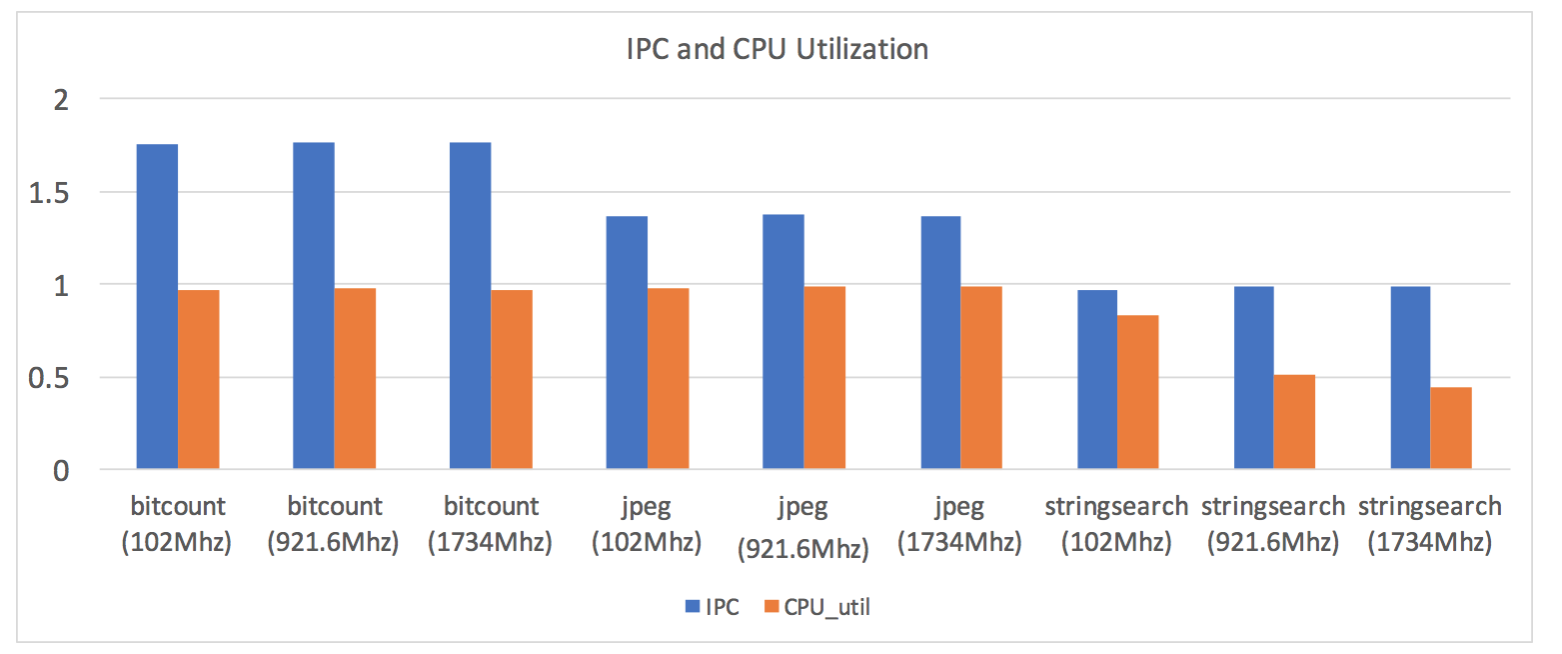
\includegraphics[width=0.5\textwidth]{cpuipc.png}
    \caption{The performance profile of CPU while running CPU benchmarks under different CPU voltage/frequency pairs.}\label{fig:cpuperf}
\end{figure}